\documentclass[11pt,a4paper]{article}
\usepackage{listings}
\usepackage{graphicx}
\usepackage[section]{placeins}
\usepackage{natbib}
\usepackage{listings}
\usepackage{float}
\usepackage[left= 1 cm,right=1cm,top=2cm,bottom=2cm]{geometry}

\title{LABWORK 6 REPORT}
\author{Ta Hoang Hai Nam - USTHBI6-110 \\ \\ Trinh Hoang Hai - USTHBI6-047 \\ \\ Le Sinh Quy - USTHBI4 -127 \\ \\ Kieu Quoc Viet - USTHBI6-153}

\begin{document}
\maketitle
\newpage 
\section{Command}

\subsection{ Install GlusterFS:}
\begin{lstlisting}
 -  Add the GlusterFS PPA repository (version 3.10):
	sudo add-apt-repository ppa:gluster/glusterfs-3.10. 
	sudo apt-get update

 -  Install GlusterFS package.
	sudo apt-get install -y glusterfs-server

\end{lstlisting}

\subsection{ Create a Trusted Pool:}

\begin{lstlisting}
 -  Get the IP Address: 
	hostname -I

 -  Add the server to the trusted pool: 
	sudo gluster peer probe <ip-address>

 -  Check the peer status
	sudo gluster peer status

\end{lstlisting}
\subsection{ Create a Distributed Replicated Volume:}
\begin{lstlisting} 
 -  Add a Storage
	For server and each node, create a folder to act as a brick.
 -  Setup a Volume
	sudo mkdir /home/<USERNAME>/gluster/test
 -  Create a Distributed Replicated Volume.
	sudo gluster volume create <VOLUME NAME> replica <INT> transport tcp <HOST NAME>:<BRICK PATH> force
 -  For instance:
	sudo gluster volume create test replica 2 transport tcp 192.168.0.160:/home/hung/gluster/test 192.168.0.175/home/lezardvaleth97/gluster/test force
 -  Start the Volume.
	sudo gluster volume start <volume name>
	sudo gluster volume start test
 -  Check the Volume status.
	sudo gluster volume info <volume name>
\end{lstlisting}
\subsection {Setup the Client}
\begin{lstlisting} 
 -  Install the GlusterFS Client.
	sudo apt-get install -y glusterfs-client
 -  Create a directory to mount the GlusterFS filesystem
 -  Mount the GlusterFS filesystem to the Client.
	sudo mount -t glusterfs <HOST IP ADDRESS>:/<VOLUME NAME> <DIRECTORY>
 -  For instance:
	sudo mount -t glusterfs 192.168.0.185:/test /mnt
 -  Verify the mounted GlusterFS filesystem.
	# df -h <mount directory>
\end{lstlisting}
\newpage 
\section{Perform Benchmarks}
\begin{lstlisting} 
 -  To perform benchmark, we send a brick with large size through gluster.
	sudo iozone -r 1024k -i 0 -i 1 -i 2 -t 4 -s 128M
	sudo iozone -r 1024k -i 0 -i 1 -i 2 -t 8 -s 128M
\end{lstlisting}
\begin{figure}[h!]
\centering
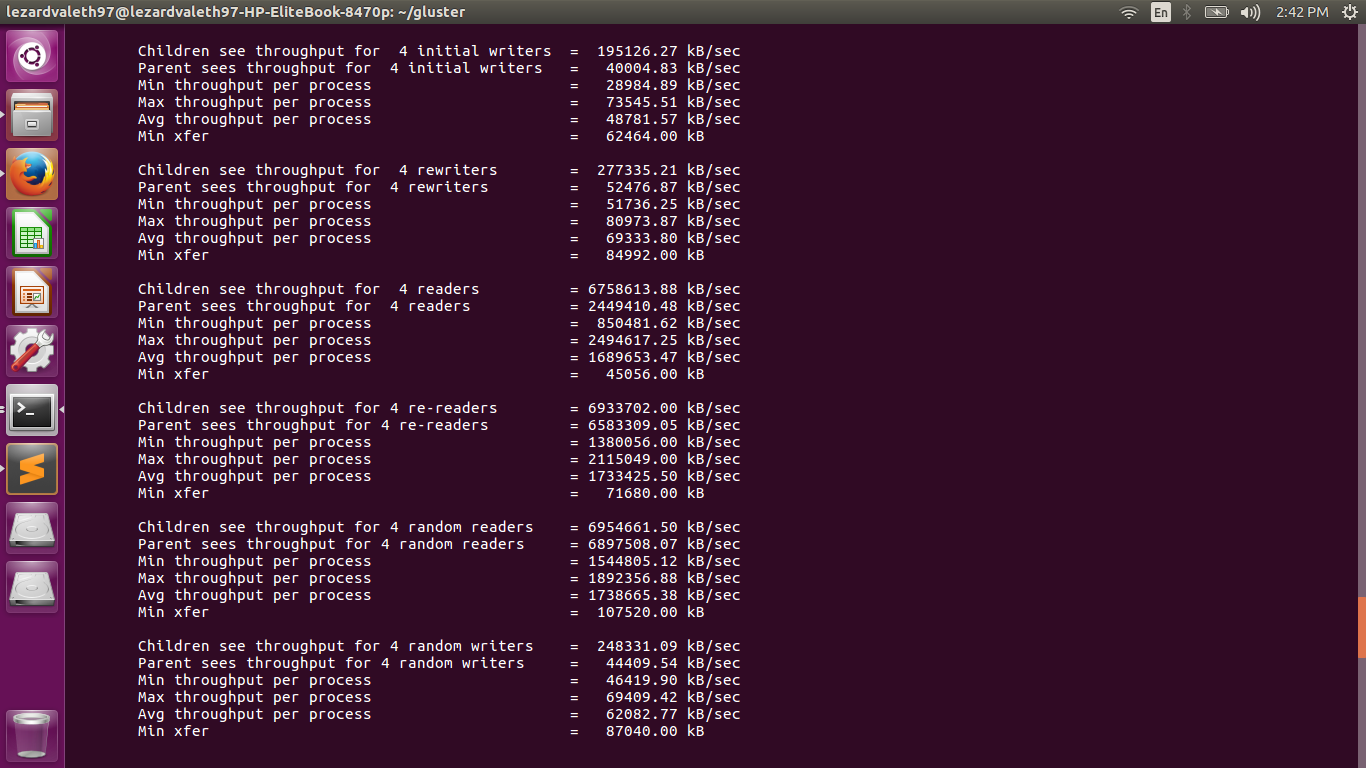
\includegraphics[scale=0.5]{1024kB_4_128M.png}
\caption{result: size 1024kB with 4 threads}

\end{figure}

\begin{figure}[h!]
\centering
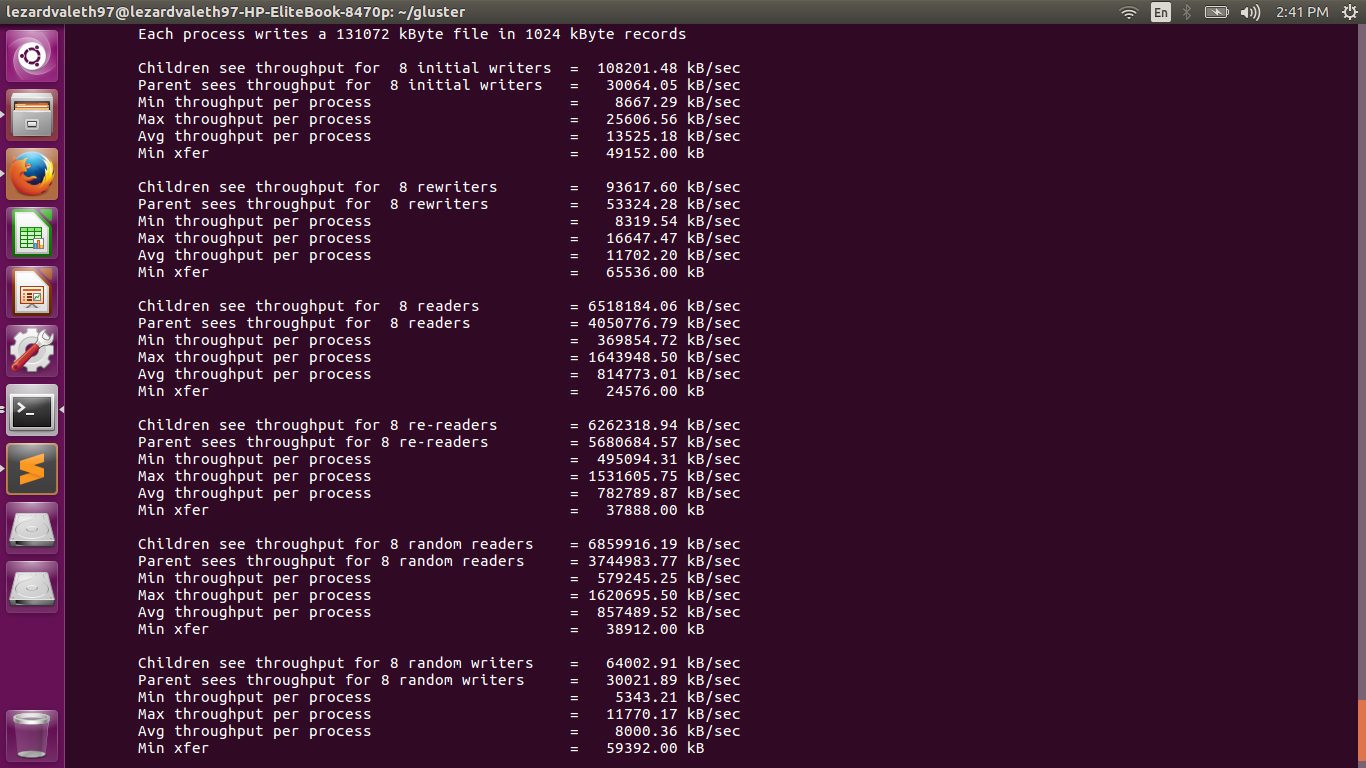
\includegraphics[scale=0.5]{1024kB_8_128M.png}
\caption{result: size 1024kB with 8 threads}
\end{figure}

\section{Who does what?}
\begin{lstlisting} 
- GlusterFS: Kieu Quoc Viet
- Report: Ta Hoang Hai Nam
\end{lstlisting}

\end{document}